\documentclass[1p]{elsarticle_modified}
%\bibliographystyle{elsarticle-num}

%\usepackage[colorlinks]{hyperref}
%\usepackage{abbrmath_seonhwa} %\Abb, \Ascr, \Acal ,\Abf, \Afrak
\usepackage{amsfonts}
\usepackage{amssymb}
\usepackage{amsmath}
\usepackage{amsthm}
\usepackage{scalefnt}
\usepackage{amsbsy}
\usepackage{kotex}
\usepackage{caption}
\usepackage{subfig}
\usepackage{color}
\usepackage{graphicx}
\usepackage{xcolor} %% white, black, red, green, blue, cyan, magenta, yellow
\usepackage{float}
\usepackage{setspace}
\usepackage{hyperref}

\usepackage{tikz}
\usetikzlibrary{arrows}

\usepackage{multirow}
\usepackage{array} % fixed length table
\usepackage{hhline}

%%%%%%%%%%%%%%%%%%%%%
\makeatletter
\renewcommand*\env@matrix[1][\arraystretch]{%
	\edef\arraystretch{#1}%
	\hskip -\arraycolsep
	\let\@ifnextchar\new@ifnextchar
	\array{*\c@MaxMatrixCols c}}
\makeatother %https://tex.stackexchange.com/questions/14071/how-can-i-increase-the-line-spacing-in-a-matrix
%%%%%%%%%%%%%%%

\usepackage[normalem]{ulem}

\newcommand{\msout}[1]{\ifmmode\text{\sout{\ensuremath{#1}}}\else\sout{#1}\fi}
%SOURCE: \msout is \stkout macro in https://tex.stackexchange.com/questions/20609/strikeout-in-math-mode

\newcommand{\cancel}[1]{
	\ifmmode
	{\color{red}\msout{#1}}
	\else
	{\color{red}\sout{#1}}
	\fi
}

\newcommand{\add}[1]{
	{\color{blue}\uwave{#1}}
}

\newcommand{\replace}[2]{
	\ifmmode
	{\color{red}\msout{#1}}{\color{blue}\uwave{#2}}
	\else
	{\color{red}\sout{#1}}{\color{blue}\uwave{#2}}
	\fi
}

\newcommand{\Sol}{\mathcal{S}} %segment
\newcommand{\D}{D} %diagram
\newcommand{\A}{\mathcal{A}} %arc


%%%%%%%%%%%%%%%%%%%%%%%%%%%%%5 test

\def\sl{\operatorname{\textup{SL}}(2,\Cbb)}
\def\psl{\operatorname{\textup{PSL}}(2,\Cbb)}
\def\quan{\mkern 1mu \triangleright \mkern 1mu}

\theoremstyle{definition}
\newtheorem{thm}{Theorem}[section]
\newtheorem{prop}[thm]{Proposition}
\newtheorem{lem}[thm]{Lemma}
\newtheorem{ques}[thm]{Question}
\newtheorem{cor}[thm]{Corollary}
\newtheorem{defn}[thm]{Definition}
\newtheorem{exam}[thm]{Example}
\newtheorem{rmk}[thm]{Remark}
\newtheorem{alg}[thm]{Algorithm}

\newcommand{\I}{\sqrt{-1}}
\begin{document}

%\begin{frontmatter}
%
%\title{Boundary parabolic representations of knots up to 8 crossings}
%
%%% Group authors per affiliation:
%\author{Yunhi Cho} 
%\address{Department of Mathematics, University of Seoul, Seoul, Korea}
%\ead{yhcho@uos.ac.kr}
%
%
%\author{Seonhwa Kim} %\fnref{s_kim}}
%\address{Center for Geometry and Physics, Institute for Basic Science, Pohang, 37673, Korea}
%\ead{ryeona17@ibs.re.kr}
%
%\author{Hyuk Kim}
%\address{Department of Mathematical Sciences, Seoul National University, Seoul 08826, Korea}
%\ead{hyukkim@snu.ac.kr}
%
%\author{Seokbeom Yoon}
%\address{Department of Mathematical Sciences, Seoul National University, Seoul, 08826,  Korea}
%\ead{sbyoon15@snu.ac.kr}
%
%\begin{abstract}
%We find all boundary parabolic representation of knots up to 8 crossings.
%
%\end{abstract}
%\begin{keyword}
%    \MSC[2010] 57M25 
%\end{keyword}
%
%\end{frontmatter}

%\linenumbers
%\tableofcontents
%
\newcommand\colored[1]{\textcolor{white}{\rule[-0.35ex]{0.8em}{1.4ex}}\kern-0.8em\color{red} #1}%
%\newcommand\colored[1]{\textcolor{white}{ #1}\kern-2.17ex	\textcolor{white}{ #1}\kern-1.81ex	\textcolor{white}{ #1}\kern-2.15ex\color{red}#1	}

{\Large $\underline{12a_{0045}~(K12a_{0045})}$}

\setlength{\tabcolsep}{10pt}
\renewcommand{\arraystretch}{1.6}
\vspace{1cm}\begin{tabular}{m{100pt}>{\centering\arraybackslash}m{274pt}}
\multirow{5}{120pt}{
	\centering
	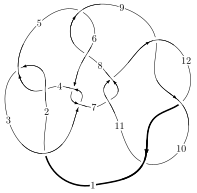
\includegraphics[width=112pt]{../../../GIT/diagram.site/Diagrams/png/846_12a_0045.png}\\
\ \ \ A knot diagram\footnotemark}&
\allowdisplaybreaks
\textbf{Linearized knot diagam} \\
\cline{2-2}
 &
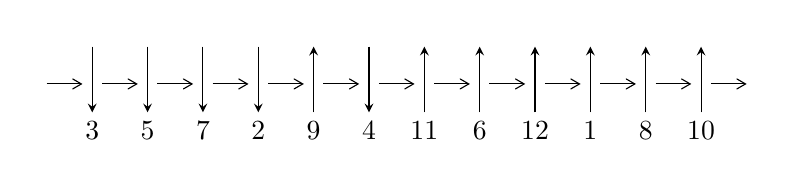
\begin{tikzpicture}[x=20pt, y=17pt]
	% nodes
	\node (C0) at (0, 0) {};
	\node (C1) at (1, 0) {};
	\node (C1U) at (1, +1) {};
	\node (C1D) at (1, -1) {3};

	\node (C2) at (2, 0) {};
	\node (C2U) at (2, +1) {};
	\node (C2D) at (2, -1) {5};

	\node (C3) at (3, 0) {};
	\node (C3U) at (3, +1) {};
	\node (C3D) at (3, -1) {7};

	\node (C4) at (4, 0) {};
	\node (C4U) at (4, +1) {};
	\node (C4D) at (4, -1) {2};

	\node (C5) at (5, 0) {};
	\node (C5U) at (5, +1) {};
	\node (C5D) at (5, -1) {9};

	\node (C6) at (6, 0) {};
	\node (C6U) at (6, +1) {};
	\node (C6D) at (6, -1) {4};

	\node (C7) at (7, 0) {};
	\node (C7U) at (7, +1) {};
	\node (C7D) at (7, -1) {11};

	\node (C8) at (8, 0) {};
	\node (C8U) at (8, +1) {};
	\node (C8D) at (8, -1) {6};

	\node (C9) at (9, 0) {};
	\node (C9U) at (9, +1) {};
	\node (C9D) at (9, -1) {12};

	\node (C10) at (10, 0) {};
	\node (C10U) at (10, +1) {};
	\node (C10D) at (10, -1) {1};

	\node (C11) at (11, 0) {};
	\node (C11U) at (11, +1) {};
	\node (C11D) at (11, -1) {8};

	\node (C12) at (12, 0) {};
	\node (C12U) at (12, +1) {};
	\node (C12D) at (12, -1) {10};
	\node (C13) at (13, 0) {};

	% arrows
	\draw[->,>={angle 60}]
	(C0) edge (C1) (C1) edge (C2) (C2) edge (C3) (C3) edge (C4) (C4) edge (C5) (C5) edge (C6) (C6) edge (C7) (C7) edge (C8) (C8) edge (C9) (C9) edge (C10) (C10) edge (C11) (C11) edge (C12) (C12) edge (C13) ;	\draw[->,>=stealth]
	(C1U) edge (C1D) (C2U) edge (C2D) (C3U) edge (C3D) (C4U) edge (C4D) (C5D) edge (C5U) (C6U) edge (C6D) (C7D) edge (C7U) (C8D) edge (C8U) (C9D) edge (C9U) (C10D) edge (C10U) (C11D) edge (C11U) (C12D) edge (C12U) ;
	\end{tikzpicture} \\
\hhline{~~} \\& 
\textbf{Solving Sequence} \\ \cline{2-2} 
 &
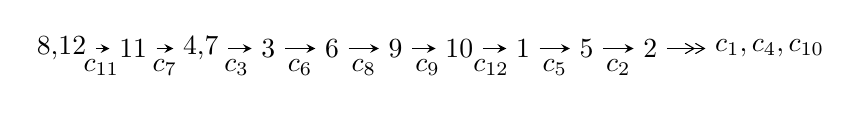
\begin{tikzpicture}[x=23pt, y=7pt]
	% node
	\node (A0) at (-1/8, 0) {8,12};
	\node (A1) at (1, 0) {11};
	\node (A2) at (33/16, 0) {4,7};
	\node (A3) at (25/8, 0) {3};
	\node (A4) at (33/8, 0) {6};
	\node (A5) at (41/8, 0) {9};
	\node (A6) at (49/8, 0) {10};
	\node (A7) at (57/8, 0) {1};
	\node (A8) at (65/8, 0) {5};
	\node (A9) at (73/8, 0) {2};
	\node (C1) at (1/2, -1) {$c_{11}$};
	\node (C2) at (3/2, -1) {$c_{7}$};
	\node (C3) at (21/8, -1) {$c_{3}$};
	\node (C4) at (29/8, -1) {$c_{6}$};
	\node (C5) at (37/8, -1) {$c_{8}$};
	\node (C6) at (45/8, -1) {$c_{9}$};
	\node (C7) at (53/8, -1) {$c_{12}$};
	\node (C8) at (61/8, -1) {$c_{5}$};
	\node (C9) at (69/8, -1) {$c_{2}$};
	\node (A10) at (11, 0) {$c_{1},c_{4},c_{10}$};

	% edge
	\draw[->,>=stealth]	
	(A0) edge (A1) (A1) edge (A2) (A2) edge (A3) (A3) edge (A4) (A4) edge (A5) (A5) edge (A6) (A6) edge (A7) (A7) edge (A8) (A8) edge (A9) ;
	\draw[->>,>={angle 60}]	
	(A9) edge (A10);
\end{tikzpicture} \\ 

\end{tabular} \\

\footnotetext{
The image of knot diagram is generated by the software ``\textbf{Draw programme}" developed by Andrew Bartholomew(\url{http://www.layer8.co.uk/maths/draw/index.htm\#Running-draw}), where we modified some parts for our purpose(\url{https://github.com/CATsTAILs/LinksPainter}).
}\phantom \\ \newline 
\centering \textbf{Ideals for irreducible components\footnotemark of $X_{\text{par}}$} 
 
\begin{align*}
I^u_{1}&=\langle 
-1.73886\times10^{473} u^{111}+7.36133\times10^{473} u^{110}+\cdots+8.44755\times10^{472} b+1.17690\times10^{476},\\
\phantom{I^u_{1}}&\phantom{= \langle  }1.22830\times10^{474} u^{111}-5.19087\times10^{474} u^{110}+\cdots+3.37902\times10^{473} a-8.06591\times10^{476},\\
\phantom{I^u_{1}}&\phantom{= \langle  }u^{112}-5 u^{111}+\cdots-5632 u+512\rangle \\
I^u_{2}&=\langle 
-3 u^7+u^6+4 u^5-3 u^4-6 u^3+2 u^2+b+3 u-4,\;4 u^7-2 u^6-5 u^5+5 u^4+7 u^3-4 u^2+a-3 u+6,\\
\phantom{I^u_{2}}&\phantom{= \langle  }u^8- u^7- u^6+2 u^5+u^4-2 u^3+2 u-1\rangle \\
I^u_{3}&=\langle 
-2 a^2 u-3 a^2+3 a u+b+4 a- u-1,\;a^3-2 a^2 u- a u+a-2 u+1,\;u^2+u-1\rangle \\
\\
I^v_{1}&=\langle 
a,\;4 v^8+372 v^7-2334 v^6+5550 v^5-4357 v^4-2618 v^3+3887 v^2+683 b+3400 v-4863,\\
\phantom{I^v_{1}}&\phantom{= \langle  }v^9-7 v^8+20 v^7-25 v^6+5 v^5+15 v^4-22 v^2+13 v+1\rangle \\
\end{align*}
\raggedright * 4 irreducible components of $\dim_{\mathbb{C}}=0$, with total 135 representations.\\
\footnotetext{All coefficients of polynomials are rational numbers. But the coefficients are sometimes approximated in decimal forms when there is not enough margin.}
\newpage
\renewcommand{\arraystretch}{1}
\centering \section*{I. $I^u_{1}= \langle -1.74\times10^{473} u^{111}+7.36\times10^{473} u^{110}+\cdots+8.45\times10^{472} b+1.18\times10^{476},\;1.23\times10^{474} u^{111}-5.19\times10^{474} u^{110}+\cdots+3.38\times10^{473} a-8.07\times10^{476},\;u^{112}-5 u^{111}+\cdots-5632 u+512 \rangle$}
\flushleft \textbf{(i) Arc colorings}\\
\begin{tabular}{m{7pt} m{180pt} m{7pt} m{180pt} }
\flushright $a_{8}=$&$\begin{pmatrix}0\\u\end{pmatrix}$ \\
\flushright $a_{12}=$&$\begin{pmatrix}1\\0\end{pmatrix}$ \\
\flushright $a_{11}=$&$\begin{pmatrix}1\\u^2\end{pmatrix}$ \\
\flushright $a_{4}=$&$\begin{pmatrix}-3.63508 u^{111}+15.3621 u^{110}+\cdots-23290.3 u+2387.06\\2.05842 u^{111}-8.71416 u^{110}+\cdots+13450.9 u-1393.18\end{pmatrix}$ \\
\flushright $a_{7}=$&$\begin{pmatrix}- u\\- u^3+u\end{pmatrix}$ \\
\flushright $a_{3}=$&$\begin{pmatrix}-3.30996 u^{111}+14.0045 u^{110}+\cdots-21203.9 u+2169.87\\1.97006 u^{111}-8.31889 u^{110}+\cdots+12707.2 u-1313.20\end{pmatrix}$ \\
\flushright $a_{6}=$&$\begin{pmatrix}0.332016 u^{111}-1.18364 u^{110}+\cdots+480.594 u-16.2789\\1.32667 u^{111}-5.42552 u^{110}+\cdots+7647.22 u-780.729\end{pmatrix}$ \\
\flushright $a_{9}=$&$\begin{pmatrix}1.36761 u^{111}-5.57410 u^{110}+\cdots+7412.94 u-742.249\\1.52926 u^{111}-6.40481 u^{110}+\cdots+9333.98 u-953.908\end{pmatrix}$ \\
\flushright $a_{10}=$&$\begin{pmatrix}2.89687 u^{111}-11.9789 u^{110}+\cdots+16746.9 u-1696.16\\1.52926 u^{111}-6.40481 u^{110}+\cdots+9333.98 u-953.908\end{pmatrix}$ \\
\flushright $a_{1}=$&$\begin{pmatrix}2.89687 u^{111}-11.9789 u^{110}+\cdots+16746.9 u-1696.16\\0.611834 u^{111}-2.49689 u^{110}+\cdots+3293.45 u-328.877\end{pmatrix}$ \\
\flushright $a_{5}=$&$\begin{pmatrix}-1.44617 u^{111}+6.03016 u^{110}+\cdots-9202.34 u+961.399\\0.0147551 u^{111}-0.115461 u^{110}+\cdots+564.279 u-65.6250\end{pmatrix}$ \\
\flushright $a_{2}=$&$\begin{pmatrix}-4.30037 u^{111}+18.0843 u^{110}+\cdots-27250.0 u+2800.12\\1.91947 u^{111}-8.15999 u^{110}+\cdots+12820.5 u-1331.36\end{pmatrix}$\\&\end{tabular}
\flushleft \textbf{(ii) Obstruction class $= -1$}\\~\\
\flushleft \textbf{(iii) Cusp Shapes $= -18.1068 u^{111}+78.6391 u^{110}+\cdots-135248. u+14140.7$}\\~\\
\newpage\renewcommand{\arraystretch}{1}
\flushleft \textbf{(iv) u-Polynomials at the component}\newline \\
\begin{tabular}{m{50pt}|m{274pt}}
Crossings & \hspace{64pt}u-Polynomials at each crossing \\
\hline $$\begin{aligned}c_{1}\end{aligned}$$&$\begin{aligned}
&u^{112}+52 u^{111}+\cdots+6550 u+1
\end{aligned}$\\
\hline $$\begin{aligned}c_{2},c_{4}\end{aligned}$$&$\begin{aligned}
&u^{112}-12 u^{111}+\cdots+78 u+1
\end{aligned}$\\
\hline $$\begin{aligned}c_{3},c_{6}\end{aligned}$$&$\begin{aligned}
&u^{112}-4 u^{111}+\cdots-1664 u+256
\end{aligned}$\\
\hline $$\begin{aligned}c_{5},c_{8}\end{aligned}$$&$\begin{aligned}
&u^{112}+3 u^{111}+\cdots-224 u-64
\end{aligned}$\\
\hline $$\begin{aligned}c_{7},c_{11}\end{aligned}$$&$\begin{aligned}
&u^{112}-5 u^{111}+\cdots-5632 u+512
\end{aligned}$\\
\hline $$\begin{aligned}c_{9},c_{10},c_{12}\end{aligned}$$&$\begin{aligned}
&u^{112}+14 u^{111}+\cdots+171 u-1
\end{aligned}$\\
\hline
\end{tabular}\\~\\
\newpage\renewcommand{\arraystretch}{1}
\flushleft \textbf{(v) Riley Polynomials at the component}\newline \\
\begin{tabular}{m{50pt}|m{274pt}}
Crossings & \hspace{64pt}Riley Polynomials at each crossing \\
\hline $$\begin{aligned}c_{1}\end{aligned}$$&$\begin{aligned}
&y^{112}+28 y^{111}+\cdots-43105022 y+1
\end{aligned}$\\
\hline $$\begin{aligned}c_{2},c_{4}\end{aligned}$$&$\begin{aligned}
&y^{112}-52 y^{111}+\cdots-6550 y+1
\end{aligned}$\\
\hline $$\begin{aligned}c_{3},c_{6}\end{aligned}$$&$\begin{aligned}
&y^{112}+60 y^{111}+\cdots-3784704 y+65536
\end{aligned}$\\
\hline $$\begin{aligned}c_{5},c_{8}\end{aligned}$$&$\begin{aligned}
&y^{112}+47 y^{111}+\cdots-185344 y+4096
\end{aligned}$\\
\hline $$\begin{aligned}c_{7},c_{11}\end{aligned}$$&$\begin{aligned}
&y^{112}-69 y^{111}+\cdots-75235328 y+262144
\end{aligned}$\\
\hline $$\begin{aligned}c_{9},c_{10},c_{12}\end{aligned}$$&$\begin{aligned}
&y^{112}-110 y^{111}+\cdots-28983 y+1
\end{aligned}$\\
\hline
\end{tabular}\\~\\
\newpage\flushleft \textbf{(vi) Complex Volumes and Cusp Shapes}
$$\begin{array}{c|c|c}  
\text{Solutions to }I^u_{1}& \I (\text{vol} + \sqrt{-1}CS) & \text{Cusp shape}\\
 \hline 
\begin{aligned}
u &= \phantom{-}0.987913 + 0.168924 I \\
a &= -0.918537 + 0.380378 I \\
b &= -0.882679 + 0.639952 I\end{aligned}
 & \phantom{-}2.30876 + 3.35064 I & \phantom{-0.000000 } 0 \\ \hline\begin{aligned}
u &= \phantom{-}0.987913 - 0.168924 I \\
a &= -0.918537 - 0.380378 I \\
b &= -0.882679 - 0.639952 I\end{aligned}
 & \phantom{-}2.30876 - 3.35064 I & \phantom{-0.000000 } 0 \\ \hline\begin{aligned}
u &= \phantom{-}0.112659 + 0.958754 I \\
a &= \phantom{-}0.550334 - 0.341976 I \\
b &= -1.17922 + 1.72177 I\end{aligned}
 & \phantom{-}1.95897 - 0.23517 I & \phantom{-0.000000 } 0 \\ \hline\begin{aligned}
u &= \phantom{-}0.112659 - 0.958754 I \\
a &= \phantom{-}0.550334 + 0.341976 I \\
b &= -1.17922 - 1.72177 I\end{aligned}
 & \phantom{-}1.95897 + 0.23517 I & \phantom{-0.000000 } 0 \\ \hline\begin{aligned}
u &= -0.941698 + 0.193747 I \\
a &= \phantom{-}0.549932 - 0.881492 I \\
b &= \phantom{-}0.117151 - 0.720063 I\end{aligned}
 & \phantom{-}4.85807 + 1.15903 I & \phantom{-0.000000 } 0 \\ \hline\begin{aligned}
u &= -0.941698 - 0.193747 I \\
a &= \phantom{-}0.549932 + 0.881492 I \\
b &= \phantom{-}0.117151 + 0.720063 I\end{aligned}
 & \phantom{-}4.85807 - 1.15903 I & \phantom{-0.000000 } 0 \\ \hline\begin{aligned}
u &= \phantom{-}0.922599 + 0.202041 I \\
a &= -0.591409 - 0.833431 I \\
b &= -0.525947 - 0.138764 I\end{aligned}
 & \phantom{-}0.14318 + 1.74876 I & \phantom{-0.000000 } 0 \\ \hline\begin{aligned}
u &= \phantom{-}0.922599 - 0.202041 I \\
a &= -0.591409 + 0.833431 I \\
b &= -0.525947 + 0.138764 I\end{aligned}
 & \phantom{-}0.14318 - 1.74876 I & \phantom{-0.000000 } 0 \\ \hline\begin{aligned}
u &= -0.989073 + 0.373226 I \\
a &= \phantom{-}0.231341 + 0.278025 I \\
b &= \phantom{-}1.082440 + 0.064268 I\end{aligned}
 & -0.37121 - 2.19836 I & \phantom{-0.000000 } 0 \\ \hline\begin{aligned}
u &= -0.989073 - 0.373226 I \\
a &= \phantom{-}0.231341 - 0.278025 I \\
b &= \phantom{-}1.082440 - 0.064268 I\end{aligned}
 & -0.37121 + 2.19836 I & \phantom{-0.000000 } 0\\
 \hline 
 \end{array}$$\newpage$$\begin{array}{c|c|c}  
\text{Solutions to }I^u_{1}& \I (\text{vol} + \sqrt{-1}CS) & \text{Cusp shape}\\
 \hline 
\begin{aligned}
u &= -1.052080 + 0.121562 I \\
a &= -0.628103 - 1.234560 I \\
b &= -0.62631 + 1.29964 I\end{aligned}
 & \phantom{-}5.22079 - 3.15983 I & \phantom{-0.000000 } 0 \\ \hline\begin{aligned}
u &= -1.052080 - 0.121562 I \\
a &= -0.628103 + 1.234560 I \\
b &= -0.62631 - 1.29964 I\end{aligned}
 & \phantom{-}5.22079 + 3.15983 I & \phantom{-0.000000 } 0 \\ \hline\begin{aligned}
u &= -0.263231 + 1.038520 I \\
a &= \phantom{-}1.031050 - 0.733739 I \\
b &= -1.21393 + 1.06445 I\end{aligned}
 & \phantom{-}5.66523 + 4.88950 I & \phantom{-0.000000 } 0 \\ \hline\begin{aligned}
u &= -0.263231 - 1.038520 I \\
a &= \phantom{-}1.031050 + 0.733739 I \\
b &= -1.21393 - 1.06445 I\end{aligned}
 & \phantom{-}5.66523 - 4.88950 I & \phantom{-0.000000 } 0 \\ \hline\begin{aligned}
u &= \phantom{-}0.919842 + 0.048399 I \\
a &= \phantom{-}1.46700 + 0.26858 I \\
b &= \phantom{-}0.767029 + 1.031570 I\end{aligned}
 & -1.49378 + 1.54613 I & \phantom{-0.000000 } 0 \\ \hline\begin{aligned}
u &= \phantom{-}0.919842 - 0.048399 I \\
a &= \phantom{-}1.46700 - 0.26858 I \\
b &= \phantom{-}0.767029 - 1.031570 I\end{aligned}
 & -1.49378 - 1.54613 I & \phantom{-0.000000 } 0 \\ \hline\begin{aligned}
u &= \phantom{-}0.313988 + 1.041330 I \\
a &= \phantom{-}2.16348 - 0.54755 I \\
b &= -3.12911 + 2.53870 I\end{aligned}
 & \phantom{-}0.16000 - 2.10599 I & \phantom{-0.000000 } 0 \\ \hline\begin{aligned}
u &= \phantom{-}0.313988 - 1.041330 I \\
a &= \phantom{-}2.16348 + 0.54755 I \\
b &= -3.12911 - 2.53870 I\end{aligned}
 & \phantom{-}0.16000 + 2.10599 I & \phantom{-0.000000 } 0 \\ \hline\begin{aligned}
u &= \phantom{-}0.859832 + 0.236554 I \\
a &= -0.32071 + 2.46620 I \\
b &= -0.76197 - 1.63661 I\end{aligned}
 & -0.994600 - 0.244702 I & \phantom{-0.000000 } 0 \\ \hline\begin{aligned}
u &= \phantom{-}0.859832 - 0.236554 I \\
a &= -0.32071 - 2.46620 I \\
b &= -0.76197 + 1.63661 I\end{aligned}
 & -0.994600 + 0.244702 I & \phantom{-0.000000 } 0\\
 \hline 
 \end{array}$$\newpage$$\begin{array}{c|c|c}  
\text{Solutions to }I^u_{1}& \I (\text{vol} + \sqrt{-1}CS) & \text{Cusp shape}\\
 \hline 
\begin{aligned}
u &= -0.645211 + 0.908882 I \\
a &= \phantom{-}0.406074 - 0.178808 I \\
b &= -0.402066 - 1.027180 I\end{aligned}
 & -4.31644 - 4.47828 I & \phantom{-0.000000 } 0 \\ \hline\begin{aligned}
u &= -0.645211 - 0.908882 I \\
a &= \phantom{-}0.406074 + 0.178808 I \\
b &= -0.402066 + 1.027180 I\end{aligned}
 & -4.31644 + 4.47828 I & \phantom{-0.000000 } 0 \\ \hline\begin{aligned}
u &= \phantom{-}1.103470 + 0.161706 I \\
a &= \phantom{-}0.356874 - 0.708417 I \\
b &= \phantom{-}1.169370 + 0.176941 I\end{aligned}
 & -0.13349 + 1.76727 I & \phantom{-0.000000 } 0 \\ \hline\begin{aligned}
u &= \phantom{-}1.103470 - 0.161706 I \\
a &= \phantom{-}0.356874 + 0.708417 I \\
b &= \phantom{-}1.169370 - 0.176941 I\end{aligned}
 & -0.13349 - 1.76727 I & \phantom{-0.000000 } 0 \\ \hline\begin{aligned}
u &= -0.869520 + 0.018980 I \\
a &= \phantom{-}0.669734 - 0.947495 I \\
b &= \phantom{-}0.19478 + 1.72833 I\end{aligned}
 & \phantom{-}4.29062 - 2.64667 I & \phantom{-0.000000 } 0 \\ \hline\begin{aligned}
u &= -0.869520 - 0.018980 I \\
a &= \phantom{-}0.669734 + 0.947495 I \\
b &= \phantom{-}0.19478 - 1.72833 I\end{aligned}
 & \phantom{-}4.29062 + 2.64667 I & \phantom{-0.000000 } 0 \\ \hline\begin{aligned}
u &= -0.097707 + 1.131780 I \\
a &= -1.26124 + 0.65545 I \\
b &= \phantom{-}1.86008 - 1.30770 I\end{aligned}
 & \phantom{-}7.06933 - 0.77487 I & \phantom{-0.000000 } 0 \\ \hline\begin{aligned}
u &= -0.097707 - 1.131780 I \\
a &= -1.26124 - 0.65545 I \\
b &= \phantom{-}1.86008 + 1.30770 I\end{aligned}
 & \phantom{-}7.06933 + 0.77487 I & \phantom{-0.000000 } 0 \\ \hline\begin{aligned}
u &= \phantom{-}1.062140 + 0.446911 I \\
a &= -0.744235 - 1.049370 I \\
b &= \phantom{-}1.011560 + 0.521470 I\end{aligned}
 & \phantom{-}3.05226 + 7.00346 I & \phantom{-0.000000 } 0 \\ \hline\begin{aligned}
u &= \phantom{-}1.062140 - 0.446911 I \\
a &= -0.744235 + 1.049370 I \\
b &= \phantom{-}1.011560 - 0.521470 I\end{aligned}
 & \phantom{-}3.05226 - 7.00346 I & \phantom{-0.000000 } 0\\
 \hline 
 \end{array}$$\newpage$$\begin{array}{c|c|c}  
\text{Solutions to }I^u_{1}& \I (\text{vol} + \sqrt{-1}CS) & \text{Cusp shape}\\
 \hline 
\begin{aligned}
u &= \phantom{-}1.116720 + 0.299470 I \\
a &= \phantom{-}0.66546 + 1.25680 I \\
b &= -0.756923 - 0.431765 I\end{aligned}
 & \phantom{-}4.78310 + 1.56650 I & \phantom{-0.000000 } 0 \\ \hline\begin{aligned}
u &= \phantom{-}1.116720 - 0.299470 I \\
a &= \phantom{-}0.66546 - 1.25680 I \\
b &= -0.756923 + 0.431765 I\end{aligned}
 & \phantom{-}4.78310 - 1.56650 I & \phantom{-0.000000 } 0 \\ \hline\begin{aligned}
u &= -0.106096 + 0.835679 I \\
a &= -1.71103 - 0.38039 I \\
b &= \phantom{-}1.45697 + 0.32666 I\end{aligned}
 & -2.60168 + 8.03413 I & \phantom{-0.000000 } 0 \\ \hline\begin{aligned}
u &= -0.106096 - 0.835679 I \\
a &= -1.71103 + 0.38039 I \\
b &= \phantom{-}1.45697 - 0.32666 I\end{aligned}
 & -2.60168 - 8.03413 I & \phantom{-0.000000 } 0 \\ \hline\begin{aligned}
u &= -1.074420 + 0.471048 I \\
a &= \phantom{-}0.48698 + 2.05471 I \\
b &= \phantom{-}2.14483 - 1.48985 I\end{aligned}
 & -2.53810 - 4.23062 I & \phantom{-0.000000 } 0 \\ \hline\begin{aligned}
u &= -1.074420 - 0.471048 I \\
a &= \phantom{-}0.48698 - 2.05471 I \\
b &= \phantom{-}2.14483 + 1.48985 I\end{aligned}
 & -2.53810 + 4.23062 I & \phantom{-0.000000 } 0 \\ \hline\begin{aligned}
u &= \phantom{-}0.750829 + 0.302715 I \\
a &= \phantom{-}0.640656 - 1.016480 I \\
b &= \phantom{-}0.600724 - 0.528679 I\end{aligned}
 & -1.53487 + 7.70823 I & \phantom{-0.000000 } 0 \\ \hline\begin{aligned}
u &= \phantom{-}0.750829 - 0.302715 I \\
a &= \phantom{-}0.640656 + 1.016480 I \\
b &= \phantom{-}0.600724 + 0.528679 I\end{aligned}
 & -1.53487 - 7.70823 I & \phantom{-0.000000 } 0 \\ \hline\begin{aligned}
u &= -0.404340 + 0.667214 I \\
a &= -2.16675 - 0.27634 I \\
b &= \phantom{-}1.38716 + 1.41067 I\end{aligned}
 & -4.57208 - 0.19764 I & \phantom{-0.000000 } 0 \\ \hline\begin{aligned}
u &= -0.404340 - 0.667214 I \\
a &= -2.16675 + 0.27634 I \\
b &= \phantom{-}1.38716 - 1.41067 I\end{aligned}
 & -4.57208 + 0.19764 I & \phantom{-0.000000 } 0\\
 \hline 
 \end{array}$$\newpage$$\begin{array}{c|c|c}  
\text{Solutions to }I^u_{1}& \I (\text{vol} + \sqrt{-1}CS) & \text{Cusp shape}\\
 \hline 
\begin{aligned}
u &= -0.562718 + 0.536308 I \\
a &= -0.119967 + 0.522623 I \\
b &= \phantom{-}0.699792 + 0.611127 I\end{aligned}
 & -1.65451 - 1.50529 I & \phantom{-0.000000 } 0 \\ \hline\begin{aligned}
u &= -0.562718 - 0.536308 I \\
a &= -0.119967 - 0.522623 I \\
b &= \phantom{-}0.699792 - 0.611127 I\end{aligned}
 & -1.65451 + 1.50529 I & \phantom{-0.000000 } 0 \\ \hline\begin{aligned}
u &= \phantom{-}0.323687 + 1.179730 I \\
a &= -0.409973 + 0.354108 I \\
b &= \phantom{-}0.60376 - 2.00524 I\end{aligned}
 & \phantom{-}1.24304 - 4.46857 I & \phantom{-0.000000 } 0 \\ \hline\begin{aligned}
u &= \phantom{-}0.323687 - 1.179730 I \\
a &= -0.409973 - 0.354108 I \\
b &= \phantom{-}0.60376 + 2.00524 I\end{aligned}
 & \phantom{-}1.24304 + 4.46857 I & \phantom{-0.000000 } 0 \\ \hline\begin{aligned}
u &= -0.962683 + 0.788038 I \\
a &= -0.260779 - 0.039002 I \\
b &= -0.405012 + 0.743652 I\end{aligned}
 & -3.38522 - 1.66545 I & \phantom{-0.000000 } 0 \\ \hline\begin{aligned}
u &= -0.962683 - 0.788038 I \\
a &= -0.260779 + 0.039002 I \\
b &= -0.405012 - 0.743652 I\end{aligned}
 & -3.38522 + 1.66545 I & \phantom{-0.000000 } 0 \\ \hline\begin{aligned}
u &= -0.287462 + 0.691754 I \\
a &= \phantom{-}0.593994 - 0.634266 I \\
b &= -0.811368 - 0.733768 I\end{aligned}
 & -4.17219 + 2.32119 I & \phantom{-0.000000 } 0 \\ \hline\begin{aligned}
u &= -0.287462 - 0.691754 I \\
a &= \phantom{-}0.593994 + 0.634266 I \\
b &= -0.811368 + 0.733768 I\end{aligned}
 & -4.17219 - 2.32119 I & \phantom{-0.000000 } 0 \\ \hline\begin{aligned}
u &= \phantom{-}1.014560 + 0.732117 I \\
a &= \phantom{-}0.215744 + 0.187366 I \\
b &= -0.010991 + 0.513589 I\end{aligned}
 & \phantom{-}1.05711 + 6.04270 I & \phantom{-0.000000 } 0 \\ \hline\begin{aligned}
u &= \phantom{-}1.014560 - 0.732117 I \\
a &= \phantom{-}0.215744 - 0.187366 I \\
b &= -0.010991 - 0.513589 I\end{aligned}
 & \phantom{-}1.05711 - 6.04270 I & \phantom{-0.000000 } 0\\
 \hline 
 \end{array}$$\newpage$$\begin{array}{c|c|c}  
\text{Solutions to }I^u_{1}& \I (\text{vol} + \sqrt{-1}CS) & \text{Cusp shape}\\
 \hline 
\begin{aligned}
u &= -1.161230 + 0.475817 I \\
a &= -0.277099 - 0.217089 I \\
b &= -1.200030 + 0.265794 I\end{aligned}
 & -1.50046 - 6.83730 I & \phantom{-0.000000 } 0 \\ \hline\begin{aligned}
u &= -1.161230 - 0.475817 I \\
a &= -0.277099 + 0.217089 I \\
b &= -1.200030 - 0.265794 I\end{aligned}
 & -1.50046 + 6.83730 I & \phantom{-0.000000 } 0 \\ \hline\begin{aligned}
u &= \phantom{-}0.447908 + 0.581740 I \\
a &= -1.18928 - 0.85724 I \\
b &= \phantom{-}0.364030 - 0.116853 I\end{aligned}
 & \phantom{-}1.18207 - 2.86004 I & \phantom{-0.000000 } 0 \\ \hline\begin{aligned}
u &= \phantom{-}0.447908 - 0.581740 I \\
a &= -1.18928 + 0.85724 I \\
b &= \phantom{-}0.364030 + 0.116853 I\end{aligned}
 & \phantom{-}1.18207 + 2.86004 I & \phantom{-0.000000 } 0 \\ \hline\begin{aligned}
u &= \phantom{-}1.284600 + 0.081267 I \\
a &= \phantom{-}0.17262 - 1.57344 I \\
b &= \phantom{-}0.216790 - 0.027700 I\end{aligned}
 & \phantom{-}4.50061 + 1.87825 I & \phantom{-0.000000 } 0 \\ \hline\begin{aligned}
u &= \phantom{-}1.284600 - 0.081267 I \\
a &= \phantom{-}0.17262 + 1.57344 I \\
b &= \phantom{-}0.216790 + 0.027700 I\end{aligned}
 & \phantom{-}4.50061 - 1.87825 I & \phantom{-0.000000 } 0 \\ \hline\begin{aligned}
u &= \phantom{-}0.814984 + 1.000110 I \\
a &= -0.255947 + 0.372325 I \\
b &= -0.65284 - 1.48503 I\end{aligned}
 & \phantom{-}0.256128 + 0.215496 I & \phantom{-0.000000 } 0 \\ \hline\begin{aligned}
u &= \phantom{-}0.814984 - 1.000110 I \\
a &= -0.255947 - 0.372325 I \\
b &= -0.65284 + 1.48503 I\end{aligned}
 & \phantom{-}0.256128 - 0.215496 I & \phantom{-0.000000 } 0 \\ \hline\begin{aligned}
u &= \phantom{-}1.061310 + 0.734995 I \\
a &= \phantom{-}0.231002 - 0.484171 I \\
b &= \phantom{-}1.28384 + 0.99105 I\end{aligned}
 & -0.08758 - 3.32486 I & \phantom{-0.000000 } 0 \\ \hline\begin{aligned}
u &= \phantom{-}1.061310 - 0.734995 I \\
a &= \phantom{-}0.231002 + 0.484171 I \\
b &= \phantom{-}1.28384 - 0.99105 I\end{aligned}
 & -0.08758 + 3.32486 I & \phantom{-0.000000 } 0\\
 \hline 
 \end{array}$$\newpage$$\begin{array}{c|c|c}  
\text{Solutions to }I^u_{1}& \I (\text{vol} + \sqrt{-1}CS) & \text{Cusp shape}\\
 \hline 
\begin{aligned}
u &= -0.140581 + 0.678756 I \\
a &= \phantom{-}1.92559 + 0.47607 I \\
b &= -1.116120 - 0.595282 I\end{aligned}
 & -0.07044 + 3.09882 I & \phantom{-0.000000 } 0 \\ \hline\begin{aligned}
u &= -0.140581 - 0.678756 I \\
a &= \phantom{-}1.92559 - 0.47607 I \\
b &= -1.116120 + 0.595282 I\end{aligned}
 & -0.07044 - 3.09882 I & \phantom{-0.000000 } 0 \\ \hline\begin{aligned}
u &= \phantom{-}0.480520 + 0.491232 I \\
a &= \phantom{-}0.479661 + 0.474885 I \\
b &= -1.358880 - 0.118546 I\end{aligned}
 & \phantom{-}1.19166 - 0.82959 I & \phantom{-0.000000 } 0 \\ \hline\begin{aligned}
u &= \phantom{-}0.480520 - 0.491232 I \\
a &= \phantom{-}0.479661 - 0.474885 I \\
b &= -1.358880 + 0.118546 I\end{aligned}
 & \phantom{-}1.19166 + 0.82959 I & \phantom{-0.000000 } 0 \\ \hline\begin{aligned}
u &= \phantom{-}0.664039 + 0.056295 I \\
a &= -2.16392 - 2.68234 I \\
b &= \phantom{-}1.22695 + 1.89143 I\end{aligned}
 & -0.844006 + 0.123701 I & \phantom{-}16.1538 - 18.4285 I \\ \hline\begin{aligned}
u &= \phantom{-}0.664039 - 0.056295 I \\
a &= -2.16392 + 2.68234 I \\
b &= \phantom{-}1.22695 - 1.89143 I\end{aligned}
 & -0.844006 - 0.123701 I & \phantom{-}16.1538 + 18.4285 I \\ \hline\begin{aligned}
u &= -1.264170 + 0.444282 I \\
a &= -0.14613 - 1.65167 I \\
b &= -1.87414 + 0.52156 I\end{aligned}
 & \phantom{-}3.43374 - 7.46948 I & \phantom{-0.000000 } 0 \\ \hline\begin{aligned}
u &= -1.264170 - 0.444282 I \\
a &= -0.14613 + 1.65167 I \\
b &= -1.87414 - 0.52156 I\end{aligned}
 & \phantom{-}3.43374 + 7.46948 I & \phantom{-0.000000 } 0 \\ \hline\begin{aligned}
u &= -1.305310 + 0.328556 I \\
a &= \phantom{-}0.89998 - 1.79680 I \\
b &= -0.91086 - 1.12171 I\end{aligned}
 & \phantom{-}5.51452 - 2.03742 I & \phantom{-0.000000 } 0 \\ \hline\begin{aligned}
u &= -1.305310 - 0.328556 I \\
a &= \phantom{-}0.89998 + 1.79680 I \\
b &= -0.91086 + 1.12171 I\end{aligned}
 & \phantom{-}5.51452 + 2.03742 I & \phantom{-0.000000 } 0\\
 \hline 
 \end{array}$$\newpage$$\begin{array}{c|c|c}  
\text{Solutions to }I^u_{1}& \I (\text{vol} + \sqrt{-1}CS) & \text{Cusp shape}\\
 \hline 
\begin{aligned}
u &= \phantom{-}0.277820 + 1.323270 I \\
a &= -1.62486 + 0.15415 I \\
b &= \phantom{-}3.25584 - 1.48744 I\end{aligned}
 & \phantom{-}6.13010 - 4.83002 I & \phantom{-0.000000 } 0 \\ \hline\begin{aligned}
u &= \phantom{-}0.277820 - 1.323270 I \\
a &= -1.62486 - 0.15415 I \\
b &= \phantom{-}3.25584 + 1.48744 I\end{aligned}
 & \phantom{-}6.13010 + 4.83002 I & \phantom{-0.000000 } 0 \\ \hline\begin{aligned}
u &= \phantom{-}1.362900 + 0.209748 I \\
a &= \phantom{-}0.02427 + 1.55962 I \\
b &= -0.574884 + 0.351957 I\end{aligned}
 & \phantom{-}2.55654 + 7.34989 I & \phantom{-0.000000 } 0 \\ \hline\begin{aligned}
u &= \phantom{-}1.362900 - 0.209748 I \\
a &= \phantom{-}0.02427 - 1.55962 I \\
b &= -0.574884 - 0.351957 I\end{aligned}
 & \phantom{-}2.55654 - 7.34989 I & \phantom{-0.000000 } 0 \\ \hline\begin{aligned}
u &= \phantom{-}1.338470 + 0.333318 I \\
a &= -0.877831 + 0.950009 I \\
b &= -2.01412 - 1.14375 I\end{aligned}
 & \phantom{-}10.99310 - 0.43900 I & \phantom{-0.000000 } 0 \\ \hline\begin{aligned}
u &= \phantom{-}1.338470 - 0.333318 I \\
a &= -0.877831 - 0.950009 I \\
b &= -2.01412 + 1.14375 I\end{aligned}
 & \phantom{-}10.99310 + 0.43900 I & \phantom{-0.000000 } 0 \\ \hline\begin{aligned}
u &= -1.316050 + 0.429456 I \\
a &= \phantom{-}0.944070 - 0.591573 I \\
b &= \phantom{-}0.66430 - 1.46767 I\end{aligned}
 & \phantom{-}6.42012 - 4.59902 I & \phantom{-0.000000 } 0 \\ \hline\begin{aligned}
u &= -1.316050 - 0.429456 I \\
a &= \phantom{-}0.944070 + 0.591573 I \\
b &= \phantom{-}0.66430 + 1.46767 I\end{aligned}
 & \phantom{-}6.42012 + 4.59902 I & \phantom{-0.000000 } 0 \\ \hline\begin{aligned}
u &= \phantom{-}0.610427\phantom{ +0.000000I} \\
a &= \phantom{-}0.610429\phantom{ +0.000000I} \\
b &= -0.200993\phantom{ +0.000000I}\end{aligned}
 & \phantom{-}0.859712\phantom{ +0.000000I} & \phantom{-}11.9150\phantom{ +0.000000I} \\ \hline\begin{aligned}
u &= \phantom{-}1.286140 + 0.548627 I \\
a &= -0.443252 + 0.043811 I \\
b &= -1.048490 - 0.319033 I\end{aligned}
 & \phantom{-}5.53294 + 5.70610 I & \phantom{-0.000000 } 0\\
 \hline 
 \end{array}$$\newpage$$\begin{array}{c|c|c}  
\text{Solutions to }I^u_{1}& \I (\text{vol} + \sqrt{-1}CS) & \text{Cusp shape}\\
 \hline 
\begin{aligned}
u &= \phantom{-}1.286140 - 0.548627 I \\
a &= -0.443252 - 0.043811 I \\
b &= -1.048490 + 0.319033 I\end{aligned}
 & \phantom{-}5.53294 - 5.70610 I & \phantom{-0.000000 } 0 \\ \hline\begin{aligned}
u &= -1.310080 + 0.531274 I \\
a &= -0.03910 + 1.65684 I \\
b &= \phantom{-}2.16792 - 0.22426 I\end{aligned}
 & \phantom{-}1.11481 - 13.24070 I & \phantom{-0.000000 } 0 \\ \hline\begin{aligned}
u &= -1.310080 - 0.531274 I \\
a &= -0.03910 - 1.65684 I \\
b &= \phantom{-}2.16792 + 0.22426 I\end{aligned}
 & \phantom{-}1.11481 + 13.24070 I & \phantom{-0.000000 } 0 \\ \hline\begin{aligned}
u &= -1.28436 + 0.61419 I \\
a &= \phantom{-}0.742337 - 1.065820 I \\
b &= -1.41432 - 0.47830 I\end{aligned}
 & \phantom{-}8.88079 - 10.89320 I & \phantom{-0.000000 } 0 \\ \hline\begin{aligned}
u &= -1.28436 - 0.61419 I \\
a &= \phantom{-}0.742337 + 1.065820 I \\
b &= -1.41432 + 0.47830 I\end{aligned}
 & \phantom{-}8.88079 + 10.89320 I & \phantom{-0.000000 } 0 \\ \hline\begin{aligned}
u &= \phantom{-}1.28360 + 0.62427 I \\
a &= -0.52411 + 1.93638 I \\
b &= -3.41369 - 1.15161 I\end{aligned}
 & \phantom{-}3.26019 + 8.19420 I & \phantom{-0.000000 } 0 \\ \hline\begin{aligned}
u &= \phantom{-}1.28360 - 0.62427 I \\
a &= -0.52411 - 1.93638 I \\
b &= -3.41369 + 1.15161 I\end{aligned}
 & \phantom{-}3.26019 - 8.19420 I & \phantom{-0.000000 } 0 \\ \hline\begin{aligned}
u &= -1.41781 + 0.19610 I \\
a &= -1.080480 + 0.444312 I \\
b &= -1.41301 + 1.02495 I\end{aligned}
 & \phantom{-}7.77601 - 0.27066 I & \phantom{-0.000000 } 0 \\ \hline\begin{aligned}
u &= -1.41781 - 0.19610 I \\
a &= -1.080480 - 0.444312 I \\
b &= -1.41301 - 1.02495 I\end{aligned}
 & \phantom{-}7.77601 + 0.27066 I & \phantom{-0.000000 } 0 \\ \hline\begin{aligned}
u &= \phantom{-}0.38913 + 1.38262 I \\
a &= \phantom{-}1.62101 + 0.04014 I \\
b &= -3.56558 + 1.43739 I\end{aligned}
 & \phantom{-}4.02685 - 10.51750 I & \phantom{-0.000000 } 0\\
 \hline 
 \end{array}$$\newpage$$\begin{array}{c|c|c}  
\text{Solutions to }I^u_{1}& \I (\text{vol} + \sqrt{-1}CS) & \text{Cusp shape}\\
 \hline 
\begin{aligned}
u &= \phantom{-}0.38913 - 1.38262 I \\
a &= \phantom{-}1.62101 - 0.04014 I \\
b &= -3.56558 - 1.43739 I\end{aligned}
 & \phantom{-}4.02685 + 10.51750 I & \phantom{-0.000000 } 0 \\ \hline\begin{aligned}
u &= -0.549537 + 0.083222 I \\
a &= \phantom{-}0.274559 - 0.934457 I \\
b &= -0.19496 + 2.94085 I\end{aligned}
 & \phantom{-}4.16876 - 2.73247 I & \phantom{-}34.1878 - 1.6499 I \\ \hline\begin{aligned}
u &= -0.549537 - 0.083222 I \\
a &= \phantom{-}0.274559 + 0.934457 I \\
b &= -0.19496 - 2.94085 I\end{aligned}
 & \phantom{-}4.16876 + 2.73247 I & \phantom{-}34.1878 + 1.6499 I \\ \hline\begin{aligned}
u &= \phantom{-}1.37781 + 0.43660 I \\
a &= \phantom{-}0.718387 - 1.203630 I \\
b &= \phantom{-}2.36665 + 1.01786 I\end{aligned}
 & \phantom{-}11.96300 + 6.19123 I & \phantom{-0.000000 } 0 \\ \hline\begin{aligned}
u &= \phantom{-}1.37781 - 0.43660 I \\
a &= \phantom{-}0.718387 + 1.203630 I \\
b &= \phantom{-}2.36665 - 1.01786 I\end{aligned}
 & \phantom{-}11.96300 - 6.19123 I & \phantom{-0.000000 } 0 \\ \hline\begin{aligned}
u &= \phantom{-}0.182434 + 0.518573 I \\
a &= \phantom{-}1.66248 + 0.93649 I \\
b &= -0.473030 - 0.208731 I\end{aligned}
 & \phantom{-}1.99985 + 1.66123 I & \phantom{-}2.31051 - 3.78283 I \\ \hline\begin{aligned}
u &= \phantom{-}0.182434 - 0.518573 I \\
a &= \phantom{-}1.66248 - 0.93649 I \\
b &= -0.473030 + 0.208731 I\end{aligned}
 & \phantom{-}1.99985 - 1.66123 I & \phantom{-}2.31051 + 3.78283 I \\ \hline\begin{aligned}
u &= -1.37397 + 0.53912 I \\
a &= -0.631049 + 1.262440 I \\
b &= \phantom{-}1.48385 + 0.78634 I\end{aligned}
 & \phantom{-}11.21670 - 5.22488 I & \phantom{-0.000000 } 0 \\ \hline\begin{aligned}
u &= -1.37397 - 0.53912 I \\
a &= -0.631049 - 1.262440 I \\
b &= \phantom{-}1.48385 - 0.78634 I\end{aligned}
 & \phantom{-}11.21670 + 5.22488 I & \phantom{-0.000000 } 0 \\ \hline\begin{aligned}
u &= \phantom{-}1.32163 + 0.66916 I \\
a &= \phantom{-}0.428382 + 0.007783 I \\
b &= \phantom{-}0.979772 + 0.650539 I\end{aligned}
 & \phantom{-}4.46415 + 11.08430 I & \phantom{-0.000000 } 0\\
 \hline 
 \end{array}$$\newpage$$\begin{array}{c|c|c}  
\text{Solutions to }I^u_{1}& \I (\text{vol} + \sqrt{-1}CS) & \text{Cusp shape}\\
 \hline 
\begin{aligned}
u &= \phantom{-}1.32163 - 0.66916 I \\
a &= \phantom{-}0.428382 - 0.007783 I \\
b &= \phantom{-}0.979772 - 0.650539 I\end{aligned}
 & \phantom{-}4.46415 - 11.08430 I & \phantom{-0.000000 } 0 \\ \hline\begin{aligned}
u &= \phantom{-}1.38900 + 0.70279 I \\
a &= \phantom{-}0.13070 - 1.64504 I \\
b &= \phantom{-}3.33755 + 0.49016 I\end{aligned}
 & \phantom{-}9.7116 + 11.9730 I & \phantom{-0.000000 } 0 \\ \hline\begin{aligned}
u &= \phantom{-}1.38900 - 0.70279 I \\
a &= \phantom{-}0.13070 + 1.64504 I \\
b &= \phantom{-}3.33755 - 0.49016 I\end{aligned}
 & \phantom{-}9.7116 - 11.9730 I & \phantom{-0.000000 } 0 \\ \hline\begin{aligned}
u &= \phantom{-}1.37841 + 0.77274 I \\
a &= \phantom{-}0.06128 + 1.66829 I \\
b &= -3.52485 - 0.31007 I\end{aligned}
 & \phantom{-}7.2346 + 18.0734 I & \phantom{-0.000000 } 0 \\ \hline\begin{aligned}
u &= \phantom{-}1.37841 - 0.77274 I \\
a &= \phantom{-}0.06128 - 1.66829 I \\
b &= -3.52485 + 0.31007 I\end{aligned}
 & \phantom{-}7.2346 - 18.0734 I & \phantom{-0.000000 } 0 \\ \hline\begin{aligned}
u &= -1.58390\phantom{ +0.000000I} \\
a &= -2.28456\phantom{ +0.000000I} \\
b &= -3.83094\phantom{ +0.000000I}\end{aligned}
 & \phantom{-}7.84469\phantom{ +0.000000I} & \phantom{-0.000000 } 0 \\ \hline\begin{aligned}
u &= -1.67053 + 0.32452 I \\
a &= \phantom{-}0.03761 + 1.53472 I \\
b &= \phantom{-}1.94736 + 1.83024 I\end{aligned}
 & \phantom{-}12.87440 - 1.42369 I & \phantom{-0.000000 } 0 \\ \hline\begin{aligned}
u &= -1.67053 - 0.32452 I \\
a &= \phantom{-}0.03761 - 1.53472 I \\
b &= \phantom{-}1.94736 - 1.83024 I\end{aligned}
 & \phantom{-}12.87440 + 1.42369 I & \phantom{-0.000000 } 0 \\ \hline\begin{aligned}
u &= -1.77832 + 0.22948 I \\
a &= -0.32455 - 1.46958 I \\
b &= -2.20973 - 2.18426 I\end{aligned}
 & \phantom{-}11.74710 + 4.07589 I & \phantom{-0.000000 } 0 \\ \hline\begin{aligned}
u &= -1.77832 - 0.22948 I \\
a &= -0.32455 + 1.46958 I \\
b &= -2.20973 + 2.18426 I\end{aligned}
 & \phantom{-}11.74710 - 4.07589 I & \phantom{-0.000000 } 0\\
 \hline 
 \end{array}$$\newpage$$\begin{array}{c|c|c}  
\text{Solutions to }I^u_{1}& \I (\text{vol} + \sqrt{-1}CS) & \text{Cusp shape}\\
 \hline 
\begin{aligned}
u &= -0.104682\phantom{ +0.000000I} \\
a &= -3.89166\phantom{ +0.000000I} \\
b &= \phantom{-}8.91953\phantom{ +0.000000I}\end{aligned}
 & \phantom{-}0.460815\phantom{ +0.000000I} & \phantom{-}373.120\phantom{ +0.000000I} \\ \hline\begin{aligned}
u &= \phantom{-}0.0766424\phantom{ +0.000000I} \\
a &= -7.27868\phantom{ +0.000000I} \\
b &= \phantom{-}0.661524\phantom{ +0.000000I}\end{aligned}
 & -1.20372\phantom{ +0.000000I} & -8.99900\phantom{ +0.000000I}\\
 \hline 
 \end{array}$$\newpage\newpage\renewcommand{\arraystretch}{1}
\centering \section*{II. $I^u_{2}= \langle -3 u^7+u^6+\cdots+b-4,\;4 u^7-2 u^6+\cdots+a+6,\;u^8- u^7- u^6+2 u^5+u^4-2 u^3+2 u-1 \rangle$}
\flushleft \textbf{(i) Arc colorings}\\
\begin{tabular}{m{7pt} m{180pt} m{7pt} m{180pt} }
\flushright $a_{8}=$&$\begin{pmatrix}0\\u\end{pmatrix}$ \\
\flushright $a_{12}=$&$\begin{pmatrix}1\\0\end{pmatrix}$ \\
\flushright $a_{11}=$&$\begin{pmatrix}1\\u^2\end{pmatrix}$ \\
\flushright $a_{4}=$&$\begin{pmatrix}-4 u^7+2 u^6+5 u^5-5 u^4-7 u^3+4 u^2+3 u-6\\3 u^7- u^6-4 u^5+3 u^4+6 u^3-2 u^2-3 u+4\end{pmatrix}$ \\
\flushright $a_{7}=$&$\begin{pmatrix}- u\\- u^3+u\end{pmatrix}$ \\
\flushright $a_{3}=$&$\begin{pmatrix}-4 u^7+2 u^6+5 u^5-5 u^4-7 u^3+4 u^2+3 u-6\\3 u^7- u^6-4 u^5+3 u^4+6 u^3-2 u^2-3 u+4\end{pmatrix}$ \\
\flushright $a_{6}=$&$\begin{pmatrix}- u\\- u^3+u\end{pmatrix}$ \\
\flushright $a_{9}=$&$\begin{pmatrix}u^3\\u^5- u^3+u\end{pmatrix}$ \\
\flushright $a_{10}=$&$\begin{pmatrix}u^5+u\\u^5- u^3+u\end{pmatrix}$ \\
\flushright $a_{1}=$&$\begin{pmatrix}u^5+u\\u^7- u^5+2 u^3- u\end{pmatrix}$ \\
\flushright $a_{5}=$&$\begin{pmatrix}- u^5- u\\- u^7+u^5-2 u^3+u\end{pmatrix}$ \\
\flushright $a_{2}=$&$\begin{pmatrix}-4 u^7+2 u^6+6 u^5-5 u^4-7 u^3+4 u^2+4 u-6\\4 u^7- u^6-5 u^5+3 u^4+8 u^3-2 u^2-4 u+4\end{pmatrix}$\\&\end{tabular}
\flushleft \textbf{(ii) Obstruction class $= 1$}\\~\\
\flushleft \textbf{(iii) Cusp Shapes $= 44 u^7-15 u^6-58 u^5+53 u^4+78 u^3-42 u^2-28 u+73$}\\~\\
\newpage\renewcommand{\arraystretch}{1}
\flushleft \textbf{(iv) u-Polynomials at the component}\newline \\
\begin{tabular}{m{50pt}|m{274pt}}
Crossings & \hspace{64pt}u-Polynomials at each crossing \\
\hline $$\begin{aligned}c_{1},c_{2}\end{aligned}$$&$\begin{aligned}
&(u-1)^8
\end{aligned}$\\
\hline $$\begin{aligned}c_{3},c_{6}\end{aligned}$$&$\begin{aligned}
&u^8
\end{aligned}$\\
\hline $$\begin{aligned}c_{4}\end{aligned}$$&$\begin{aligned}
&(u+1)^8
\end{aligned}$\\
\hline $$\begin{aligned}c_{5}\end{aligned}$$&$\begin{aligned}
&u^8+3 u^7+7 u^6+10 u^5+11 u^4+10 u^3+6 u^2+4 u+1
\end{aligned}$\\
\hline $$\begin{aligned}c_{7}\end{aligned}$$&$\begin{aligned}
&u^8+u^7- u^6-2 u^5+u^4+2 u^3-2 u-1
\end{aligned}$\\
\hline $$\begin{aligned}c_{8}\end{aligned}$$&$\begin{aligned}
&u^8-3 u^7+7 u^6-10 u^5+11 u^4-10 u^3+6 u^2-4 u+1
\end{aligned}$\\
\hline $$\begin{aligned}c_{9},c_{10}\end{aligned}$$&$\begin{aligned}
&u^8- u^7-3 u^6+2 u^5+3 u^4-2 u-1
\end{aligned}$\\
\hline $$\begin{aligned}c_{11}\end{aligned}$$&$\begin{aligned}
&u^8- u^7- u^6+2 u^5+u^4-2 u^3+2 u-1
\end{aligned}$\\
\hline $$\begin{aligned}c_{12}\end{aligned}$$&$\begin{aligned}
&u^8+u^7-3 u^6-2 u^5+3 u^4+2 u-1
\end{aligned}$\\
\hline
\end{tabular}\\~\\
\newpage\renewcommand{\arraystretch}{1}
\flushleft \textbf{(v) Riley Polynomials at the component}\newline \\
\begin{tabular}{m{50pt}|m{274pt}}
Crossings & \hspace{64pt}Riley Polynomials at each crossing \\
\hline $$\begin{aligned}c_{1},c_{2},c_{4}\end{aligned}$$&$\begin{aligned}
&(y-1)^8
\end{aligned}$\\
\hline $$\begin{aligned}c_{3},c_{6}\end{aligned}$$&$\begin{aligned}
&y^8
\end{aligned}$\\
\hline $$\begin{aligned}c_{5},c_{8}\end{aligned}$$&$\begin{aligned}
&y^8+5 y^7+11 y^6+6 y^5-17 y^4-34 y^3-22 y^2-4 y+1
\end{aligned}$\\
\hline $$\begin{aligned}c_{7},c_{11}\end{aligned}$$&$\begin{aligned}
&y^8-3 y^7+7 y^6-10 y^5+11 y^4-10 y^3+6 y^2-4 y+1
\end{aligned}$\\
\hline $$\begin{aligned}c_{9},c_{10},c_{12}\end{aligned}$$&$\begin{aligned}
&y^8-7 y^7+19 y^6-22 y^5+3 y^4+14 y^3-6 y^2-4 y+1
\end{aligned}$\\
\hline
\end{tabular}\\~\\
\newpage\flushleft \textbf{(vi) Complex Volumes and Cusp Shapes}
$$\begin{array}{c|c|c}  
\text{Solutions to }I^u_{2}& \I (\text{vol} + \sqrt{-1}CS) & \text{Cusp shape}\\
 \hline 
\begin{aligned}
u &= \phantom{-}0.570868 + 0.730671 I \\
a &= \phantom{-}1.145920 + 0.510212 I \\
b &= -1.80990 + 0.33963 I\end{aligned}
 & -0.604279 - 1.131230 I & \phantom{-}0.744211 - 0.553382 I \\ \hline\begin{aligned}
u &= \phantom{-}0.570868 - 0.730671 I \\
a &= \phantom{-}1.145920 - 0.510212 I \\
b &= -1.80990 - 0.33963 I\end{aligned}
 & -0.604279 + 1.131230 I & \phantom{-}0.744211 + 0.553382 I \\ \hline\begin{aligned}
u &= -0.855237 + 0.665892 I \\
a &= -0.315815 + 0.718986 I \\
b &= \phantom{-}1.043770 - 0.152194 I\end{aligned}
 & -3.80435 - 2.57849 I & -2.39106 + 4.72239 I \\ \hline\begin{aligned}
u &= -0.855237 - 0.665892 I \\
a &= -0.315815 - 0.718986 I \\
b &= \phantom{-}1.043770 + 0.152194 I\end{aligned}
 & -3.80435 + 2.57849 I & -2.39106 - 4.72239 I \\ \hline\begin{aligned}
u &= -1.09818\phantom{ +0.000000I} \\
a &= \phantom{-}0.755058\phantom{ +0.000000I} \\
b &= \phantom{-}0.155540\phantom{ +0.000000I}\end{aligned}
 & \phantom{-}4.85780\phantom{ +0.000000I} & \phantom{-}8.45210\phantom{ +0.000000I} \\ \hline\begin{aligned}
u &= \phantom{-}1.031810 + 0.655470 I \\
a &= \phantom{-}0.069364 + 0.543055 I \\
b &= -0.759875 - 0.104398 I\end{aligned}
 & \phantom{-}0.73474 + 6.44354 I & \phantom{-}0.47538 - 9.99765 I \\ \hline\begin{aligned}
u &= \phantom{-}1.031810 - 0.655470 I \\
a &= \phantom{-}0.069364 - 0.543055 I \\
b &= -0.759875 + 0.104398 I\end{aligned}
 & \phantom{-}0.73474 - 6.44354 I & \phantom{-}0.47538 + 9.99765 I \\ \hline\begin{aligned}
u &= \phantom{-}0.603304\phantom{ +0.000000I} \\
a &= -4.55399\phantom{ +0.000000I} \\
b &= \phantom{-}2.89645\phantom{ +0.000000I}\end{aligned}
 & -0.799899\phantom{ +0.000000I} & \phantom{-}60.8910\phantom{ +0.000000I}\\
 \hline 
 \end{array}$$\newpage\newpage\renewcommand{\arraystretch}{1}
\centering \section*{III. $I^u_{3}= \langle -2 a^2 u-3 a^2+3 a u+b+4 a- u-1,\;a^3-2 a^2 u- a u+a-2 u+1,\;u^2+u-1 \rangle$}
\flushleft \textbf{(i) Arc colorings}\\
\begin{tabular}{m{7pt} m{180pt} m{7pt} m{180pt} }
\flushright $a_{8}=$&$\begin{pmatrix}0\\u\end{pmatrix}$ \\
\flushright $a_{12}=$&$\begin{pmatrix}1\\0\end{pmatrix}$ \\
\flushright $a_{11}=$&$\begin{pmatrix}1\\- u+1\end{pmatrix}$ \\
\flushright $a_{4}=$&$\begin{pmatrix}a\\2 a^2 u+3 a^2-3 a u-4 a+u+1\end{pmatrix}$ \\
\flushright $a_{7}=$&$\begin{pmatrix}- u\\- u+1\end{pmatrix}$ \\
\flushright $a_{3}=$&$\begin{pmatrix}a^2 u+a^2- a+u\\2 a^2 u+2 a^2- a u-4 a+2 u\end{pmatrix}$ \\
\flushright $a_{6}=$&$\begin{pmatrix}0\\2 a^2 u+3 a^2- a u-2 a- u-1\end{pmatrix}$ \\
\flushright $a_{9}=$&$\begin{pmatrix}0\\u\end{pmatrix}$ \\
\flushright $a_{10}=$&$\begin{pmatrix}u\\u\end{pmatrix}$ \\
\flushright $a_{1}=$&$\begin{pmatrix}u\\u-1\end{pmatrix}$ \\
\flushright $a_{5}=$&$\begin{pmatrix}0\\2 a^2 u+3 a^2- a u-2 a- u-1\end{pmatrix}$ \\
\flushright $a_{2}=$&$\begin{pmatrix}a^2 u+a^2- a+u\\2 a^2 u+2 a^2-2 a-2\end{pmatrix}$\\&\end{tabular}
\flushleft \textbf{(ii) Obstruction class $= 1$}\\~\\
\flushleft \textbf{(iii) Cusp Shapes $= 19 a^2 u+23 a^2-17 a u-29 a+3 u+1$}\\~\\
\newpage\renewcommand{\arraystretch}{1}
\flushleft \textbf{(iv) u-Polynomials at the component}\newline \\
\begin{tabular}{m{50pt}|m{274pt}}
Crossings & \hspace{64pt}u-Polynomials at each crossing \\
\hline $$\begin{aligned}c_{1},c_{3}\end{aligned}$$&$\begin{aligned}
&(u^3- u^2+2 u-1)^2
\end{aligned}$\\
\hline $$\begin{aligned}c_{2}\end{aligned}$$&$\begin{aligned}
&(u^3+u^2-1)^2
\end{aligned}$\\
\hline $$\begin{aligned}c_{4}\end{aligned}$$&$\begin{aligned}
&(u^3- u^2+1)^2
\end{aligned}$\\
\hline $$\begin{aligned}c_{5},c_{8}\end{aligned}$$&$\begin{aligned}
&u^6
\end{aligned}$\\
\hline $$\begin{aligned}c_{6}\end{aligned}$$&$\begin{aligned}
&(u^3+u^2+2 u+1)^2
\end{aligned}$\\
\hline $$\begin{aligned}c_{7},c_{9},c_{10}\end{aligned}$$&$\begin{aligned}
&(u^2- u-1)^3
\end{aligned}$\\
\hline $$\begin{aligned}c_{11},c_{12}\end{aligned}$$&$\begin{aligned}
&(u^2+u-1)^3
\end{aligned}$\\
\hline
\end{tabular}\\~\\
\newpage\renewcommand{\arraystretch}{1}
\flushleft \textbf{(v) Riley Polynomials at the component}\newline \\
\begin{tabular}{m{50pt}|m{274pt}}
Crossings & \hspace{64pt}Riley Polynomials at each crossing \\
\hline $$\begin{aligned}c_{1},c_{3},c_{6}\end{aligned}$$&$\begin{aligned}
&(y^3+3 y^2+2 y-1)^2
\end{aligned}$\\
\hline $$\begin{aligned}c_{2},c_{4}\end{aligned}$$&$\begin{aligned}
&(y^3- y^2+2 y-1)^2
\end{aligned}$\\
\hline $$\begin{aligned}c_{5},c_{8}\end{aligned}$$&$\begin{aligned}
&y^6
\end{aligned}$\\
\hline $$\begin{aligned}c_{7},c_{9},c_{10}\\c_{11},c_{12}\end{aligned}$$&$\begin{aligned}
&(y^2-3 y+1)^3
\end{aligned}$\\
\hline
\end{tabular}\\~\\
\newpage\flushleft \textbf{(vi) Complex Volumes and Cusp Shapes}
$$\begin{array}{c|c|c}  
\text{Solutions to }I^u_{3}& \I (\text{vol} + \sqrt{-1}CS) & \text{Cusp shape}\\
 \hline 
\begin{aligned}
u &= \phantom{-}0.618034\phantom{ +0.000000I} \\
a &= \phantom{-}1.08457\phantom{ +0.000000I} \\
b &= \phantom{-}0.251717\phantom{ +0.000000I}\end{aligned}
 & -0.126494\phantom{ +0.000000I} & \phantom{-}0.874100\phantom{ +0.000000I} \\ \hline\begin{aligned}
u &= \phantom{-}0.618034\phantom{ +0.000000I} \\
a &= \phantom{-}0.075747 + 0.460350 I \\
b &= \phantom{-}0.30119 - 2.39951 I\end{aligned}
 & \phantom{-}4.01109 + 2.82812 I & -7.3018 - 15.7639 I \\ \hline\begin{aligned}
u &= \phantom{-}0.618034\phantom{ +0.000000I} \\
a &= \phantom{-}0.075747 - 0.460350 I \\
b &= \phantom{-}0.30119 + 2.39951 I\end{aligned}
 & \phantom{-}4.01109 - 2.82812 I & -7.3018 + 15.7639 I \\ \hline\begin{aligned}
u &= -1.61803\phantom{ +0.000000I} \\
a &= -0.198308 + 1.205210 I \\
b &= -0.453796 + 1.142220 I\end{aligned}
 & \phantom{-}11.90680 - 2.82812 I & \phantom{-}7.38403 + 1.90115 I \\ \hline\begin{aligned}
u &= -1.61803\phantom{ +0.000000I} \\
a &= -0.198308 - 1.205210 I \\
b &= -0.453796 - 1.142220 I\end{aligned}
 & \phantom{-}11.90680 + 2.82812 I & \phantom{-}7.38403 - 1.90115 I \\ \hline\begin{aligned}
u &= -1.61803\phantom{ +0.000000I} \\
a &= -2.83945\phantom{ +0.000000I} \\
b &= -4.94651\phantom{ +0.000000I}\end{aligned}
 & \phantom{-}7.76919\phantom{ +0.000000I} & -62.0390\phantom{ +0.000000I}\\
 \hline 
 \end{array}$$\newpage\newpage\renewcommand{\arraystretch}{1}
\centering \section*{IV. $I^v_{1}= \langle a,\;4 v^8+372 v^7+\cdots+683 b-4863,\;v^9-7 v^8+\cdots+13 v+1 \rangle$}
\flushleft \textbf{(i) Arc colorings}\\
\begin{tabular}{m{7pt} m{180pt} m{7pt} m{180pt} }
\flushright $a_{8}=$&$\begin{pmatrix}v\\0\end{pmatrix}$ \\
\flushright $a_{12}=$&$\begin{pmatrix}1\\0\end{pmatrix}$ \\
\flushright $a_{11}=$&$\begin{pmatrix}1\\0\end{pmatrix}$ \\
\flushright $a_{4}=$&$\begin{pmatrix}0\\-0.00585652 v^{8}-0.544656 v^{7}+\cdots-4.97804 v+7.12006\end{pmatrix}$ \\
\flushright $a_{7}=$&$\begin{pmatrix}v\\0\end{pmatrix}$ \\
\flushright $a_{3}=$&$\begin{pmatrix}-0.565154 v^{8}+3.44070 v^{7}+\cdots+7.61933 v+0.585652\\-0.00585652 v^{8}-0.544656 v^{7}+\cdots-4.97804 v+7.12006\end{pmatrix}$ \\
\flushright $a_{6}=$&$\begin{pmatrix}v\\0.595900 v^{8}-3.58126 v^{7}+\cdots-7.48463 v+3.28404\end{pmatrix}$ \\
\flushright $a_{9}=$&$\begin{pmatrix}-1.00439 v^{8}+5.59151 v^{7}+\cdots+9.26647 v+0.590044\\1\end{pmatrix}$ \\
\flushright $a_{10}=$&$\begin{pmatrix}-1.00439 v^{8}+5.59151 v^{7}+\cdots+9.26647 v+1.59004\\1\end{pmatrix}$ \\
\flushright $a_{1}=$&$\begin{pmatrix}1.00439 v^{8}-5.59151 v^{7}+\cdots-9.26647 v-0.590044\\-1\end{pmatrix}$ \\
\flushright $a_{5}=$&$\begin{pmatrix}-1.00439 v^{8}+5.59151 v^{7}+\cdots+9.26647 v+0.590044\\0.00585652 v^{8}-0.455344 v^{7}+\cdots-3.02196 v+3.87994\end{pmatrix}$ \\
\flushright $a_{2}=$&$\begin{pmatrix}0.569546 v^{8}-3.03221 v^{7}+\cdots-3.88580 v-0.175695\\0.00585652 v^{8}-0.455344 v^{7}+\cdots-3.02196 v+3.87994\end{pmatrix}$\\&\end{tabular}
\flushleft \textbf{(ii) Obstruction class $= 1$}\\~\\
\flushleft \textbf{(iii) Cusp Shapes $= -\frac{8299}{683} v^8+\frac{59404}{683} v^7-\frac{175193}{683} v^6+\frac{233079}{683} v^5-\frac{71022}{683} v^4-\frac{122802}{683} v^3+\frac{17898}{683} v^2+\frac{188382}{683} v-\frac{131415}{683}$}\\~\\
\newpage\renewcommand{\arraystretch}{1}
\flushleft \textbf{(iv) u-Polynomials at the component}\newline \\
\begin{tabular}{m{50pt}|m{274pt}}
Crossings & \hspace{64pt}u-Polynomials at each crossing \\
\hline $$\begin{aligned}c_{1}\end{aligned}$$&$\begin{aligned}
&u^9-5 u^8+12 u^7-15 u^6+9 u^5+u^4-4 u^3+2 u^2+u-1
\end{aligned}$\\
\hline $$\begin{aligned}c_{2}\end{aligned}$$&$\begin{aligned}
&u^9+u^8-2 u^7-3 u^6+u^5+3 u^4+2 u^3- u-1
\end{aligned}$\\
\hline $$\begin{aligned}c_{3}\end{aligned}$$&$\begin{aligned}
&u^9+u^8+2 u^7+u^6+3 u^5+u^4+2 u^3+u-1
\end{aligned}$\\
\hline $$\begin{aligned}c_{4}\end{aligned}$$&$\begin{aligned}
&u^9- u^8-2 u^7+3 u^6+u^5-3 u^4+2 u^3- u+1
\end{aligned}$\\
\hline $$\begin{aligned}c_{5}\end{aligned}$$&$\begin{aligned}
&u^9+3 u^8+8 u^7+13 u^6+17 u^5+17 u^4+12 u^3+6 u^2+u-1
\end{aligned}$\\
\hline $$\begin{aligned}c_{6}\end{aligned}$$&$\begin{aligned}
&u^9- u^8+2 u^7- u^6+3 u^5- u^4+2 u^3+u+1
\end{aligned}$\\
\hline $$\begin{aligned}c_{7},c_{11}\end{aligned}$$&$\begin{aligned}
&u^9
\end{aligned}$\\
\hline $$\begin{aligned}c_{8}\end{aligned}$$&$\begin{aligned}
&u^9-3 u^8+8 u^7-13 u^6+17 u^5-17 u^4+12 u^3-6 u^2+u+1
\end{aligned}$\\
\hline $$\begin{aligned}c_{9},c_{10}\end{aligned}$$&$\begin{aligned}
&(u+1)^9
\end{aligned}$\\
\hline $$\begin{aligned}c_{12}\end{aligned}$$&$\begin{aligned}
&(u-1)^9
\end{aligned}$\\
\hline
\end{tabular}\\~\\
\newpage\renewcommand{\arraystretch}{1}
\flushleft \textbf{(v) Riley Polynomials at the component}\newline \\
\begin{tabular}{m{50pt}|m{274pt}}
Crossings & \hspace{64pt}Riley Polynomials at each crossing \\
\hline $$\begin{aligned}c_{1}\end{aligned}$$&$\begin{aligned}
&y^9- y^8+12 y^7-7 y^6+37 y^5+y^4-10 y^2+5 y-1
\end{aligned}$\\
\hline $$\begin{aligned}c_{2},c_{4}\end{aligned}$$&$\begin{aligned}
&y^9-5 y^8+12 y^7-15 y^6+9 y^5+y^4-4 y^3+2 y^2+y-1
\end{aligned}$\\
\hline $$\begin{aligned}c_{3},c_{6}\end{aligned}$$&$\begin{aligned}
&y^9+3 y^8+8 y^7+13 y^6+17 y^5+17 y^4+12 y^3+6 y^2+y-1
\end{aligned}$\\
\hline $$\begin{aligned}c_{5},c_{8}\end{aligned}$$&$\begin{aligned}
&y^9+7 y^8+20 y^7+25 y^6+5 y^5-15 y^4+22 y^2+13 y-1
\end{aligned}$\\
\hline $$\begin{aligned}c_{7},c_{11}\end{aligned}$$&$\begin{aligned}
&y^9
\end{aligned}$\\
\hline $$\begin{aligned}c_{9},c_{10},c_{12}\end{aligned}$$&$\begin{aligned}
&(y-1)^9
\end{aligned}$\\
\hline
\end{tabular}\\~\\
\newpage\flushleft \textbf{(vi) Complex Volumes and Cusp Shapes}
$$\begin{array}{c|c|c}  
\text{Solutions to }I^v_{1}& \I (\text{vol} + \sqrt{-1}CS) & \text{Cusp shape}\\
 \hline 
\begin{aligned}
v &= -0.763784 + 0.496693 I \\
a &= \phantom{-0.000000 } 0 \\
b &= -0.449406 + 0.973624 I\end{aligned}
 & \phantom{-}3.42837 - 2.09337 I & \phantom{-}7.68972 + 3.82038 I \\ \hline\begin{aligned}
v &= -0.763784 - 0.496693 I \\
a &= \phantom{-0.000000 } 0 \\
b &= -0.449406 - 0.973624 I\end{aligned}
 & \phantom{-}3.42837 + 2.09337 I & \phantom{-}7.68972 - 3.82038 I \\ \hline\begin{aligned}
v &= \phantom{-}1.072290 + 0.815867 I \\
a &= \phantom{-0.000000 } 0 \\
b &= -0.764470 - 0.234457 I\end{aligned}
 & \phantom{-}1.02799 - 2.45442 I & \phantom{-}5.04100 + 1.69416 I \\ \hline\begin{aligned}
v &= \phantom{-}1.072290 - 0.815867 I \\
a &= \phantom{-0.000000 } 0 \\
b &= -0.764470 + 0.234457 I\end{aligned}
 & \phantom{-}1.02799 + 2.45442 I & \phantom{-}5.04100 - 1.69416 I \\ \hline\begin{aligned}
v &= \phantom{-}1.353070 + 0.224375 I \\
a &= \phantom{-0.000000 } 0 \\
b &= \phantom{-}0.485105 - 0.622283 I\end{aligned}
 & -2.72642 - 1.33617 I & -1.56769 + 0.26615 I \\ \hline\begin{aligned}
v &= \phantom{-}1.353070 - 0.224375 I \\
a &= \phantom{-0.000000 } 0 \\
b &= \phantom{-}0.485105 + 0.622283 I\end{aligned}
 & -2.72642 + 1.33617 I & -1.56769 - 0.26615 I \\ \hline\begin{aligned}
v &= -0.0689118\phantom{ +0.000000I} \\
a &= \phantom{-0.000000 } 0 \\
b &= \phantom{-}7.43498\phantom{ +0.000000I}\end{aligned}
 & \phantom{-}0.446489\phantom{ +0.000000I} & -211.240\phantom{ +0.000000I} \\ \hline\begin{aligned}
v &= \phantom{-}1.87288 + 1.26938 I \\
a &= \phantom{-0.000000 } 0 \\
b &= \phantom{-}0.511281 + 0.180088 I\end{aligned}
 & -1.95319 - 7.08493 I & \phantom{-}0.45449 + 1.34000 I \\ \hline\begin{aligned}
v &= \phantom{-}1.87288 - 1.26938 I \\
a &= \phantom{-0.000000 } 0 \\
b &= \phantom{-}0.511281 - 0.180088 I\end{aligned}
 & -1.95319 + 7.08493 I & \phantom{-}0.45449 - 1.34000 I\\
 \hline 
 \end{array}$$\newpage
\newpage\renewcommand{\arraystretch}{1}
\centering \section*{ V. u-Polynomials}
\begin{tabular}{m{50pt}|m{274pt}}
Crossings & \hspace{64pt}u-Polynomials at each crossing \\
\hline $$\begin{aligned}c_{1}\end{aligned}$$&$\begin{aligned}
&(u-1)^8(u^3- u^2+2 u-1)^2\\
&\cdot(u^9-5 u^8+12 u^7-15 u^6+9 u^5+u^4-4 u^3+2 u^2+u-1)\\
&\cdot(u^{112}+52 u^{111}+\cdots+6550 u+1)
\end{aligned}$\\
\hline $$\begin{aligned}c_{2}\end{aligned}$$&$\begin{aligned}
&(u-1)^8(u^3+u^2-1)^2(u^9+u^8-2 u^7-3 u^6+u^5+3 u^4+2 u^3- u-1)\\
&\cdot(u^{112}-12 u^{111}+\cdots+78 u+1)
\end{aligned}$\\
\hline $$\begin{aligned}c_{3}\end{aligned}$$&$\begin{aligned}
&u^8(u^3- u^2+2 u-1)^2(u^9+u^8+2 u^7+u^6+3 u^5+u^4+2 u^3+u-1)\\
&\cdot(u^{112}-4 u^{111}+\cdots-1664 u+256)
\end{aligned}$\\
\hline $$\begin{aligned}c_{4}\end{aligned}$$&$\begin{aligned}
&(u+1)^8(u^3- u^2+1)^2(u^9- u^8-2 u^7+3 u^6+u^5-3 u^4+2 u^3- u+1)\\
&\cdot(u^{112}-12 u^{111}+\cdots+78 u+1)
\end{aligned}$\\
\hline $$\begin{aligned}c_{5}\end{aligned}$$&$\begin{aligned}
&u^6(u^8+3 u^7+7 u^6+10 u^5+11 u^4+10 u^3+6 u^2+4 u+1)\\
&\cdot(u^9+3 u^8+8 u^7+13 u^6+17 u^5+17 u^4+12 u^3+6 u^2+u-1)\\
&\cdot(u^{112}+3 u^{111}+\cdots-224 u-64)
\end{aligned}$\\
\hline $$\begin{aligned}c_{6}\end{aligned}$$&$\begin{aligned}
&u^8(u^3+u^2+2 u+1)^2(u^9- u^8+2 u^7- u^6+3 u^5- u^4+2 u^3+u+1)\\
&\cdot(u^{112}-4 u^{111}+\cdots-1664 u+256)
\end{aligned}$\\
\hline $$\begin{aligned}c_{7}\end{aligned}$$&$\begin{aligned}
&u^9(u^2- u-1)^3(u^8+u^7- u^6-2 u^5+u^4+2 u^3-2 u-1)\\
&\cdot(u^{112}-5 u^{111}+\cdots-5632 u+512)
\end{aligned}$\\
\hline $$\begin{aligned}c_{8}\end{aligned}$$&$\begin{aligned}
&u^6(u^8-3 u^7+7 u^6-10 u^5+11 u^4-10 u^3+6 u^2-4 u+1)\\
&\cdot(u^9-3 u^8+8 u^7-13 u^6+17 u^5-17 u^4+12 u^3-6 u^2+u+1)\\
&\cdot(u^{112}+3 u^{111}+\cdots-224 u-64)
\end{aligned}$\\
\hline $$\begin{aligned}c_{9},c_{10}\end{aligned}$$&$\begin{aligned}
&(u+1)^9(u^2- u-1)^3(u^8- u^7-3 u^6+2 u^5+3 u^4-2 u-1)\\
&\cdot(u^{112}+14 u^{111}+\cdots+171 u-1)
\end{aligned}$\\
\hline $$\begin{aligned}c_{11}\end{aligned}$$&$\begin{aligned}
&u^9(u^2+u-1)^3(u^8- u^7- u^6+2 u^5+u^4-2 u^3+2 u-1)\\
&\cdot(u^{112}-5 u^{111}+\cdots-5632 u+512)
\end{aligned}$\\
\hline $$\begin{aligned}c_{12}\end{aligned}$$&$\begin{aligned}
&(u-1)^9(u^2+u-1)^3(u^8+u^7-3 u^6-2 u^5+3 u^4+2 u-1)\\
&\cdot(u^{112}+14 u^{111}+\cdots+171 u-1)
\end{aligned}$\\
\hline
\end{tabular}\newpage\renewcommand{\arraystretch}{1}
\centering \section*{ VI. Riley Polynomials}
\begin{tabular}{m{50pt}|m{274pt}}
Crossings & \hspace{64pt}Riley Polynomials at each crossing \\
\hline $$\begin{aligned}c_{1}\end{aligned}$$&$\begin{aligned}
&(y-1)^8(y^3+3 y^2+2 y-1)^2\\
&\cdot(y^9- y^8+12 y^7-7 y^6+37 y^5+y^4-10 y^2+5 y-1)\\
&\cdot(y^{112}+28 y^{111}+\cdots-43105022 y+1)
\end{aligned}$\\
\hline $$\begin{aligned}c_{2},c_{4}\end{aligned}$$&$\begin{aligned}
&(y-1)^8(y^3- y^2+2 y-1)^2\\
&\cdot(y^9-5 y^8+12 y^7-15 y^6+9 y^5+y^4-4 y^3+2 y^2+y-1)\\
&\cdot(y^{112}-52 y^{111}+\cdots-6550 y+1)
\end{aligned}$\\
\hline $$\begin{aligned}c_{3},c_{6}\end{aligned}$$&$\begin{aligned}
&y^8(y^3+3 y^2+2 y-1)^2\\
&\cdot(y^9+3 y^8+8 y^7+13 y^6+17 y^5+17 y^4+12 y^3+6 y^2+y-1)\\
&\cdot(y^{112}+60 y^{111}+\cdots-3784704 y+65536)
\end{aligned}$\\
\hline $$\begin{aligned}c_{5},c_{8}\end{aligned}$$&$\begin{aligned}
&y^6(y^8+5 y^7+11 y^6+6 y^5-17 y^4-34 y^3-22 y^2-4 y+1)\\
&\cdot(y^9+7 y^8+20 y^7+25 y^6+5 y^5-15 y^4+22 y^2+13 y-1)\\
&\cdot(y^{112}+47 y^{111}+\cdots-185344 y+4096)
\end{aligned}$\\
\hline $$\begin{aligned}c_{7},c_{11}\end{aligned}$$&$\begin{aligned}
&y^9(y^2-3 y+1)^3(y^8-3 y^7+\cdots-4 y+1)\\
&\cdot(y^{112}-69 y^{111}+\cdots-75235328 y+262144)
\end{aligned}$\\
\hline $$\begin{aligned}c_{9},c_{10},c_{12}\end{aligned}$$&$\begin{aligned}
&(y-1)^9(y^2-3 y+1)^3\\
&\cdot(y^8-7 y^7+19 y^6-22 y^5+3 y^4+14 y^3-6 y^2-4 y+1)\\
&\cdot(y^{112}-110 y^{111}+\cdots-28983 y+1)
\end{aligned}$\\
\hline
\end{tabular}
\vskip 2pc
\end{document}